\documentclass[aps,prd,onecolumn,amsmath,amssymb,nofootinbib,superscriptaddress]{revtex4-2}
% Preprint, not peer reviewed.  Version 2026-06-11 (v2; v1 was 2026-06-04).

\usepackage{amsmath,amssymb}
\usepackage{graphicx}

\begin{document}

\title{Non-Markovian Gravitational Decoherence: A Gaussian-Onset Alternative to the
Di\'osi--Penrose Exponential}

\author{Felix Robles Elvira}
\thanks{ORCID: 0009-0009-2017-4394.  Independent researcher.}
\noaffiliation

\date{Version of 11 June 2026 --- preprint, not peer reviewed}

\begin{abstract}
Gravitationally induced decoherence, in the Di\'osi--Penrose (DP) form, predicts that a spatial
superposition of a massive body loses coherence at a rate set by the gravitational self-energy
$E_G$ of the mass-density difference between the branches, with characteristic time
$\tau_G=\hbar/E_G$. The DP law is exponential in time, a form that follows from an implicit
Markov (memoryless, divisible) assumption about the underlying stochastic dynamics. We examine
gravitational decoherence within the framework of \emph{indivisible stochastic processes} (ISP)
of Barandes, whose defining feature is the failure of the divisibility (Chapman--Kolmogorov)
property. Indivisibility motivates treating the gravitational record-mismatch noise as
non-Markovian (finite memory time $\tau_c$) rather than white. ISP motivates this finite-memory
replacement, and an explicit division-event model (Sec.~\ref{subsec:micro}) grounds the resulting
exponential kernel and pins $\tau_c$---modulo one stated ansatz, with the energy scale inherited
from DP. We show
that any such finite-memory noise---a finite, regular covariance with no white component---generically
replaces the DP exponential with a non-exponential coherence decay whose short-time exponent is
quadratic: Gaussian, $C(T)=C(0)\exp[-\tfrac12(T/\tau_G)^2]$, when the mismatch-energy fluctuation
scale is of order $E_G$ and $\tau_c$ is at least of order $\tau_G$, crossing over to a DP-slope
exponential tail at later times. The strict DP exponential is recovered in the white-noise limit
($\tau_c\to0$ at fixed noise power), where the Gaussian onset window closes. The distinction is
experimentally sharp and \emph{rate-robust} (it does not rely on fitting a single exponential
rate): the onset shape of the residual gravitational log-coherence is linear in $T$ for Markovian
collapse and quadratic (zero initial slope, a Zeno-like plateau) for the indivisible case. We give
threshold masses and separations for levitated-nanosphere, matter-wave, and mechanical-cat-state
platforms, set out differential strategies (notably a density lever and common-mode subtraction) to
separate the gravitational onset from environmental backgrounds, and confront the radiation and heating
bounds, which constrain only the model's regularization length---the per-nucleon emission
($\propto 1/R_0^3$), decoupled from the ($R_0$-independent) collective decoherence the interferometer
measures ($\propto GM^2/R$)---so the finite-memory modification changes the \emph{onset shape}, not the
radiation phenomenology. We are explicit about scope: the quadratic onset is the
generic signature of non-Markovian decoherence and is shared with other coloured-noise collapse
models, so the test falsifies \emph{strict} Markovian DP/CSL and would be evidence for a
non-Markovian fundamental channel consistent with ISP, but does not by itself single out ISP.
\end{abstract}

\maketitle

\section{Introduction}\label{sec:intro}

The persistence of quantum coherence for increasingly massive systems is one of the sharpest open
questions at the quantum--classical and quantum--gravity interfaces. Objective-collapse models
posit a fundamental, observer-independent mechanism that suppresses macroscopic superpositions
\cite{R4,R5,R6,R7}. Among them, the proposals of Di\'osi~\cite{R2,R3} and Penrose~\cite{R1} tie
this suppression specifically to gravity: a superposition of two distinct mass distributions is a
superposition of two distinct spacetime geometries, and the gravitational self-energy of their
difference sets a decoherence time $\tau_G=\hbar/E_G$. This ``Di\'osi--Penrose'' (DP) decoherence
is now an active experimental target, both directly through matter-wave and optomechanical
interferometry~\cite{R16,R19,R23,R26,R27} and indirectly through spontaneous-radiation
searches~\cite{R8,R9}, the latter having already excluded the simplest, parameter-free DP
model~\cite{R8}.

The DP coherence law is exponential, $C(T)=C(0)\exp(-T/\tau_G)$. This functional form is not an
independent prediction of gravity; it is a consequence of treating the underlying collapse noise as
\emph{white} (delta-correlated in time), equivalently of assuming the reduced dynamics forms a
Markovian semigroup. White noise is an idealization~\cite{R10}, and the open-systems literature
shows that non-Markovian (coloured) environments generically produce non-exponential coherence
decay, with a universal quadratic (Zeno-like) onset at short times~\cite{R15,R21,R22}.

In this paper we ask what gravitational decoherence looks like when the underlying dynamics is
taken to be \emph{indivisible} in the sense of Barandes' stochastic-quantum
correspondence~\cite{R11,R12}. An indivisible stochastic process is one whose transition law does
\emph{not} factorize through intermediate times,
\begin{equation}
\Gamma(t_2,t_0)\neq\Gamma(t_2,t_1)\,\Gamma(t_1,t_0),
\end{equation}
i.e.\ it violates exactly the divisibility property that underlies the Markovian semigroup. Our
central result is that this feature---finite memory in the gravitational channel---replaces the DP
exponential with a non-exponential law whose short-time exponent is quadratic (Gaussian when the
fluctuation scale is of order $E_G$), and that the difference is experimentally accessible through a
\emph{shape-based} onset measurement that needs no fitted rate. We recover the DP exponential in the
white-noise (Markovian) limit, identify the new time scale $\tau_c$ that controls the crossover, and
confront the existing spontaneous-radiation bound.

Our claims are deliberately bounded. Indivisibility \emph{motivates} a finite-memory gravitational
channel; an explicit division-event model (Sec.~\ref{subsec:micro}) then grounds the exponential
kernel and pins $\tau_c$, at the cost of one stated ansatz, while the amplitude (energy scale) is
inherited from DP. The mechanism is a \emph{reconstruction} of gravitational decoherence within a
particular stochastic ontology, and the new, falsifiable content is the non-exponential onset, not
the energy scale. The
quadratic onset is the generic signature of non-Markovianity and is not unique to ISP. The robust,
central claim is that the DP exponential is a Markovian idealization and that finite memory yields a
falsifiable onset-shape discriminator; the radiation and heating bounds (Sec.~\ref{sec:radiation})
constrain only the model's regularization length and decouple from the ($R_0$-independent) decoherence,
so they do not threaten the prediction. We make these
limitations explicit in Sec.~\ref{sec:limits}.

\section{Indivisible stochastic dynamics and the record-stabilization hypothesis}\label{sec:isp}

Barandes' stochastic-quantum correspondence~\cite{R11,R12} establishes that a broad class of quantum
systems can be represented as stochastic processes over a configuration space in which the
configuration is a definite quantity (``beable'') at all times, with the unitary, Hilbert-space
description emerging as an exact reformulation. The processes that correspond to generic quantum
evolution are \emph{indivisible}: their transition matrices do not satisfy the Chapman--Kolmogorov
composition law except at isolated \emph{division events}, times at which the process momentarily
factorizes and behaves Markovianly. Division events are, in this picture, the natural locus of
effective measurement and record formation~\cite{R11,R12}.

We adopt the following hypothesis, consistent with this picture and with the gravitational-decoherence
proposals~\cite{R1,R2,R3,R20}: when two coherent branches carry distinct effective mass-density
records, the gravitational distinguishability of the corresponding geometries acts as a channel that
\emph{stabilizes} the branches into distinct records. The stabilization is not a primitive collapse
postulate; it is the statement that the gravitational mismatch supplies a positive, accumulating
``cost'' that suppresses the survival of the unstabilized (coherent) alternative. We make this
quantitative in the next two sections and emphasise where the indivisible structure changes the
result.

We distinguish three physically separate effects, only the third of which is the subject of this paper:
\begin{enumerate}
\item \textbf{Environmental decoherence}---ordinary scattering, gas collisions, thermal emission;
reducible in principle by better isolation~\cite{R14,R16}.
\item \textbf{Unitary gravitational phase}---gravity shifts the relative phase of the branches
without destroying coherence.
\item \textbf{Gravitational record stabilization}---the geometric mismatch itself acts as a
branch-stabilizing (decohering) channel. This is the putative new physics.
\end{enumerate}

\section{Gravitational mismatch energy and the Markovian (Di\'osi--Penrose) limit}\label{sec:dp}

Let the two branches carry mass densities $\rho_r(x)$ and $\rho_{r'}(x)$, with difference
$\delta\rho(x)=\rho_r(x)-\rho_{r'}(x)$. Following Di\'osi and Penrose~\cite{R1,R2,R3}, the
gravitational mismatch energy is the Newtonian self-energy of the difference,
\begin{equation}
E_G=\frac{G}{2}\int d^3x\,d^3y\;\frac{\delta\rho(x)\,\delta\rho(y)}{|x-y|}.
\end{equation}
$E_G$ is non-negative once a finite object size is retained; the point-mass limit is not admissible
because it diverges, exactly the regularization issue that the experimental bounds constrain
\cite{R8}. Define the dimensionless gravitational action accumulated over a hold time $T$,
\begin{equation}
a(T)=\frac{E_G\,T}{\hbar},\qquad \tau_G=\frac{\hbar}{E_G}.
\end{equation}
The standard DP result is the exponential coherence law
\begin{equation}
C(T)=C(0)\,\exp(-T/\tau_G).
\end{equation}
It is instructive to see precisely which assumption produces the exponential. Write the survival
factor $S(E_G,T)=|C(T)|/|C(0)|$. If one assumes (i) time multiplicativity $S(E_G,T+U)=S(E_G,T)\,
S(E_G,U)$ and (ii) dependence only on the dimensionless action $a$ (additivity of independent cost
channels then follows and need not be assumed separately), the Cauchy functional equation forces
\begin{equation}
S=\exp(-\kappa\,a)=\exp(-\kappa\,E_G T/\hbar),
\end{equation}
with the coefficient $\kappa$ fixed by normalization. Assumption (i) is the semigroup
(Chapman--Kolmogorov) property: it states that processing over the whole interval factorizes into
independent processing over its parts. \textbf{This is the divisibility / Markov assumption.} (This
functional argument is not the historical derivation of DP, which follows from a Markovian master
equation~\cite{R2,R20}; it serves only to isolate the semigroup assumption behind \emph{any}
exponential survival law.) The DP exponential is therefore the Markovian special case of a more
general survival functional. We now drop assumption (i), as the indivisible structure requires.

\section{Indivisible dynamics and non-exponential decoherence}\label{sec:indiv}

\subsection{A minimal finite-memory model}\label{subsec:model}

Indivisibility motivates \emph{finite memory}, but a specific coherence law needs an explicit model.
We state one as a benchmark and label every assumption, since not all of them come from ISP. Let the
relative phase between the branches accumulate from a real gravitational record-mismatch energy
$\delta E(t)$,
\begin{equation}
\varphi(T)=\frac{1}{\hbar}\int_0^T \delta E(t)\,dt,\qquad
\frac{C(T)}{C(0)}=\big\langle e^{i\varphi(T)}\big\rangle,
\end{equation}
and posit:
\begin{itemize}
\item \textbf{(M1) Gaussian, stationary noise---standard.} $\delta E(t)$ is a stationary Gaussian
process with covariance $K(s)=\mathrm{Cov}[\delta E(t),\delta E(t+s)]$; then the cumulant expansion
truncates at second order and the coherence modulus is $|\langle e^{i\varphi}\rangle|=\exp(-\tfrac12
\,\mathrm{Var}\,\varphi)$ exactly (any nonzero mean of $\delta E$ contributes only the unitary phase
of Sec.~\ref{sec:isp}). This is the ordinary Gaussian-dephasing model, not specific to ISP.
\item \textbf{(M2) Amplitude set by $E_G$---the DP ansatz.} The fluctuation scale is the
gravitational self-energy of the mass-density difference, $\sigma_E\sim E_G$. Note $\delta E$ is a
genuine \emph{fluctuation}, not a definite phase rate: a definite $\delta E$ would give only the
unitary phase of Sec.~\ref{sec:isp}, and it is the \emph{randomness} of $\delta E$ that decoheres.
That the gravitational self-energy of a superposition is \emph{indefinite}---hence a noise of scale
$E_G$ rather than a phase---is the Di\'osi--Penrose hypothesis, taken over unchanged.
\item \textbf{(M3) Finite memory---the ISP-motivated part.} $K(s)$ has a finite correlation
(record-memory) time $\tau_c$ and is \emph{not} white. This is the one ingredient indivisibility
supplies: a non-divisible process does not decorrelate instantaneously, so the white-noise
idealization underlying DP is dropped.
\end{itemize}

Under (M1) the coherence obeys the standard second-cumulant decoherence functional~\cite{R15,R21}
(we write the decoherence exponent $\chi(T)$, reserving $\Gamma$ for Barandes' transition matrix)
\begin{equation}
\ln\frac{|C(T)|}{|C(0)|}=-\,\chi(T),\qquad
\chi(T)=\frac{1}{2\hbar^2}\int_0^T\!\!\int_0^T K(t_1-t_2)\,dt_1\,dt_2 .
\end{equation}
It is convenient to name the \emph{noise power} $D_E\equiv\sigma_E^2\,\tau_c$, so the zero-frequency
weight is $S(0)=\int K\,ds=2D_E$. Only (M3) is ISP's; (M1) is standard and (M2) is DP's, and
everything below is the consequence of (M3)---that $K$ is not white---for the \emph{shape} of $C(T)$.
Two limits bracket the behaviour.

\paragraph{Markovian (white-noise) limit} ($\tau_c\to0$ at fixed noise power $D_E$, so
$K\to2D_E\,\delta$): the double integral is linear in $T$, $\chi(T)=(D_E/\hbar^2)\,T$, recovering the
DP exponential and identifying $1/\tau_G=E_G/\hbar$ when $D_E=E_G\hbar$. This limit fixes the
\emph{power}, not the amplitude: as $\tau_c\to0$, $\sigma_E\to\infty$.

\paragraph{Fully-correlated limit} ($\tau_c\to\infty$, an idealized limit in which the hold spans a
single indivisible transition with no internal decorrelation---not the literal content of
indivisibility, which is only the failure of factorization): here it is instead the \emph{amplitude}
$\sigma_E$ that is held fixed, $K\approx\sigma_E^2$ is constant, so
\begin{equation}
\chi(T)=\tfrac12\Big(\frac{\sigma_E T}{\hbar}\Big)^2,
\end{equation}
a quadratic exponent and hence a Gaussian coherence decay.

\subsection{The prediction hierarchy}\label{subsec:hierarchy}

It helps to separate what finite memory \emph{forces} from what the benchmark closure \emph{adds}.

\paragraph{Generic finite-memory onset---closure-independent.} Expanding the functional for
$T\ll\tau_c$, where $K(t_1-t_2)\approx\sigma_E^2$, gives a quadratic exponent
\begin{equation}
\boxed{\,\chi(T)=\frac{\sigma_E^2}{2\hbar^2}\,T^2 + \text{higher order},\,}
\end{equation}
a \emph{zero-initial-slope} decay whatever the kernel's detailed shape. This is the robust,
falsifiable content; it does not depend on identifying $\sigma_E$ with $E_G$.

\paragraph{Benchmark closure.} The two scales are fixed by the self-consistent closure (derived in
Sec.~\ref{subsec:micro} from the division-event model), $\sigma_E\sim E_G$ and $\tau_c\sim\tau_G$---the
unique closure built from the single available scale $E_G$ (its only time is $\hbar/E_G$, its only
energy $E_G$), reinforced by the argument that the record-memory time equals the stabilization time.

\paragraph{Benchmark prediction.} In the onset region $T\lesssim\tau_c$ the closure gives a Gaussian
at DP's scale,
\begin{equation}
\boxed{\,C(T)=C(0)\,\exp\!\Big[-\tfrac12\,(T/\tau_G)^2\Big],\qquad \tau_G=\hbar/E_G,\,}
\end{equation}
crossing over to a DP-slope exponential tail at later times.

For a generic finite $\tau_c$ with the exponential memory kernel $K(s)=\sigma_E^2\,e^{-|s|/\tau_c}$
the full closed form is
\begin{equation}
\chi(T)=\frac{\sigma_E^2\,\tau_c^2}{\hbar^2}\Big(\frac{T}{\tau_c}-1+e^{-T/\tau_c}\Big),
\end{equation}
Gaussian for $T\ll\tau_c$ and linear (DP-slope) for $T\gg\tau_c$. The long-time slope is set by the
noise power $D_E=\sigma_E^2\,\tau_c$, the onset curvature by the amplitude $\sigma_E^2$, so the
Gaussian onset time is $\tau_{\rm Gauss}=\sqrt{\tau_c\,\tau_G}$, equal to $\tau_G$ only at the
closure $\tau_c\sim\tau_G$. One must therefore \emph{not} recover DP by taking $\tau_c\to0$ at fixed
$\sigma_E$, where the slope vanishes; the strict DP exponential is the white-noise limit ($D_E$ held
at $E_G\hbar$, $\tau_c\to0$, $\sigma_E\to\infty$), in which the Gaussian onset window closes. (The
divergent amplitude $\sigma_E\to\infty$ of that limit is the source of white-noise DP's ultraviolet
radiation problem; a finite $\tau_c$ band-limits the noise in time---a \emph{temporal} regulator
complementary to DP's \emph{spatial} regularization $R_0$, see Sec.~\ref{sec:radiation}.) At the
closure $D_E=E_G\hbar$ automatically, so the late-time tail carries exactly the DP slope $1/\tau_G$:
a single self-consistent law (Gaussian onset, DP-slope tail, crossover at $\tau_G$), not a
one-parameter interpolation at fixed amplitude.

The short-time quadratic onset is not an artefact of the exponential kernel; it is the universal
consequence of finite-correlation-time (smooth) noise, identical in origin to the quantum-Zeno
short-time behaviour of any open system~\cite{R22}, and is required by $\chi'(0)=0$ whenever the
noise has no white (delta) component.

\paragraph{What is forced, inherited, and assumed.} In sum: the \emph{quadratic onset} (zero initial
slope) is forced by finite memory (M3); the \emph{energy scale} $E_G$ is inherited from
Di\'osi--Penrose (M2); the \emph{Gaussian form at} $\tau_G$ follows only after the benchmark closure.
The model is therefore a finite-memory, DP-family phenomenology \emph{motivated} by ISP---not a
first-principles derivation of the memory kernel from indivisible dynamics.

\subsection{A microscopic division-event model}\label{subsec:micro}

The exponential kernel and the scale $\tau_c$ need not be assumed---both follow from an explicit
indivisible model of the channel. Model the gravitational record channel as a \emph{renewal-reset}
process: $\delta E(t)$ is held constant between Barandes division events and redrawn (the record
stabilizing) at each, with division events forming a renewal process of mean spacing $\tau_c$. The
stationary autocovariance is then
\begin{equation}
K(s) = \sigma_E^2\,P_{\rm same}(s),\qquad
P_{\rm same}(s) = \frac{1}{\tau_c}\int_s^{\infty}(\tau-s)\,\psi(\tau)\,d\tau,
\end{equation}
fixed by the division-waiting-time law $\psi$. \textbf{Memoryless (Poisson) division events give
exactly the exponential kernel} $K(s)=\sigma_E^2 e^{-|s|/\tau_c}$ assumed above, with $\tau_c$ the mean
inter-division time; regular divisions give instead a triangular kernel---so the kernel shape encodes
the division statistics, a microstructure that colored-noise CSL lacks.

The scale $\tau_c$ is then fixed self-consistently rather than dimensionally: a division event
\emph{is} a record stabilization, which occurs once the channel has accumulated order-unity
decoherence, $\chi(\tau_c)\approx1$. With $\sigma_E\sim E_G$,
\begin{equation}
\chi(\tau_c)=\Big(\frac{\tau_c}{\tau_G}\Big)^2 e^{-1}=1 \;\Longrightarrow\; \tau_c\approx1.65\,\tau_G,
\tag{closure}
\end{equation}
pinning the crossover to $\tau_G$ (see Sec.~\ref{sec:tauc} for the alternative candidate scales). This
converts the two inputs of Secs.~\ref{subsec:model}--\ref{subsec:hierarchy}---the exponential kernel and
$\tau_c\sim\tau_G$---into consequences of a single assumption: that the gravitational record channel
undergoes memoryless division events.

We are explicit that the renewal-reset dynamics is itself a model. It makes Barandes' division events
concrete and reproduces the kernel, but deriving it from the full configuration-space indivisible
process for a gravitationally-coupled system remains open. So this grounds the kernel one level
deeper---in the division-event structure---without claiming a first-principles derivation.

(One bookkeeping caveat on the closure: the renewal-reset process is a jump process, not jointly
Gaussian, so the second-cumulant $\chi$ used in the closure is exact only to the same
$O(10\%)$ non-Gaussian corrections quantified in the third-axis discussion; the fixed point
$\tau_c \approx 1.65\,\tau_G$ inherits that accuracy, which is ample for its role as a scale
estimate.)

\paragraph{On the state-dependence this introduces.} Because $\tau_c\approx1.65\,\tau_G\propto1/E_G$,
the record-memory time scales with the experimentally-chosen mass configuration. This is \emph{not} a
dynamical backreaction or a Schr\"odinger--Newton nonlinearity: $\chi(\tau_c)\approx1$ is an algebraic
self-consistency condition that fixes a parameter once $E_G$ is given, not a self-potential sourced by
the wavefunction (the mean-field Schr\"odinger--Newton effect is a deterministic phase \emph{shift}
with no decay---a separate entry in the Sec.~\ref{sec:disc} classification, testable by the
proposed optomechanical Schr\"odinger--Newton experiments~\cite{R24}). For a fixed preparation the dynamics is an ordinary \emph{linear} dephasing
channel, and the $E_G$-dependence of $\tau_c$ is the same kind of state-dependence as the
$E_G$-dependence of the decay \emph{rate} $1/\tau_G$ in standard DP/CSL. What differs is the
bookkeeping: DP/CSL obtain that dependence as an \emph{emergent} matrix element of a master equation
with state-independent coefficients ($R_0$, $\lambda$), whereas here $\tau_c$ is fixed \emph{from} the
two-branch $E_G$. The relation $\tau_c\sim\tau_G$ is therefore an \textbf{effective, two-branch
description}---adequate for the interferometric test, where $E_G$ is a fixed number---and not yet a
fundamental, state-independent law for arbitrary (multi-branch, continuous) superpositions; supplying
that law is part of the same open problem as grounding the division dynamics in Barandes' formalism.

\section{A shape-based interferometric discriminator}\label{sec:disc}

The practical signature is the \emph{shape} of the decay near $T=0$; the discriminating feature is
its leading power in $T$, which is \emph{rate-robust}---it does not rely on an absolute collapse-rate
fit. Prepare a spatial superposition with fixed gravitational mismatch $E_G$ and a fixed
environmental budget $\Gamma_{\rm env}$, and measure the interferometric visibility $V(T)$. Define
the residual gravitational log-coherence by subtracting the separately measured environmental
contribution (cleanly, by the density lever below --- same size, shape and surface at lower bulk
density; the cruder $E_G\to0$ small-separation control changes the environmental rate too, since
$\Gamma_{\rm env}$ itself depends on $d$ below the environment's coherence wavelength, and is
usable only with that $d$-dependence modeled out),
\begin{equation}
L(T)=\ln\frac{V(T)}{V_{\rm env}(T)}.
\end{equation}
The three hypotheses give qualitatively distinct onsets:
\begin{equation}
L(T)=
\begin{cases}
0, & \text{ordinary quantum mechanics (no fundamental channel),}\\[2pt]
-\,T/\tau_G, & \text{Markovian collapse: finite initial slope (rate shown for DP; CSL's rate is set by $(\lambda, r_C)$),}\\[2pt]
-\,\tfrac12(T/\tau_G)^2, & \text{indivisible ISP: zero initial slope (parabola tangent to axis).}
\end{cases}
\end{equation}
The discriminator is therefore: a straight line through the origin $\Rightarrow$ Markovian DP/CSL; a
parabola tangent at the origin $\Rightarrow$ indivisible ISP (Fig.~\ref{fig:onset}). Because the
shape (linear vs quadratic onset) is independent of the overall coefficient, the test does not
require knowing $\tau_G$ in advance, nor the absolute collapse strength---only the ability to vary
$E_G$ while holding the environment fixed, and to resolve the curvature of $L(T)$ at small $T$
(distinguishing a small linear slope from a small quadratic curvature is itself a statistical task,
but one that needs no absolute-rate calibration).

\begin{figure}[t]
\centering
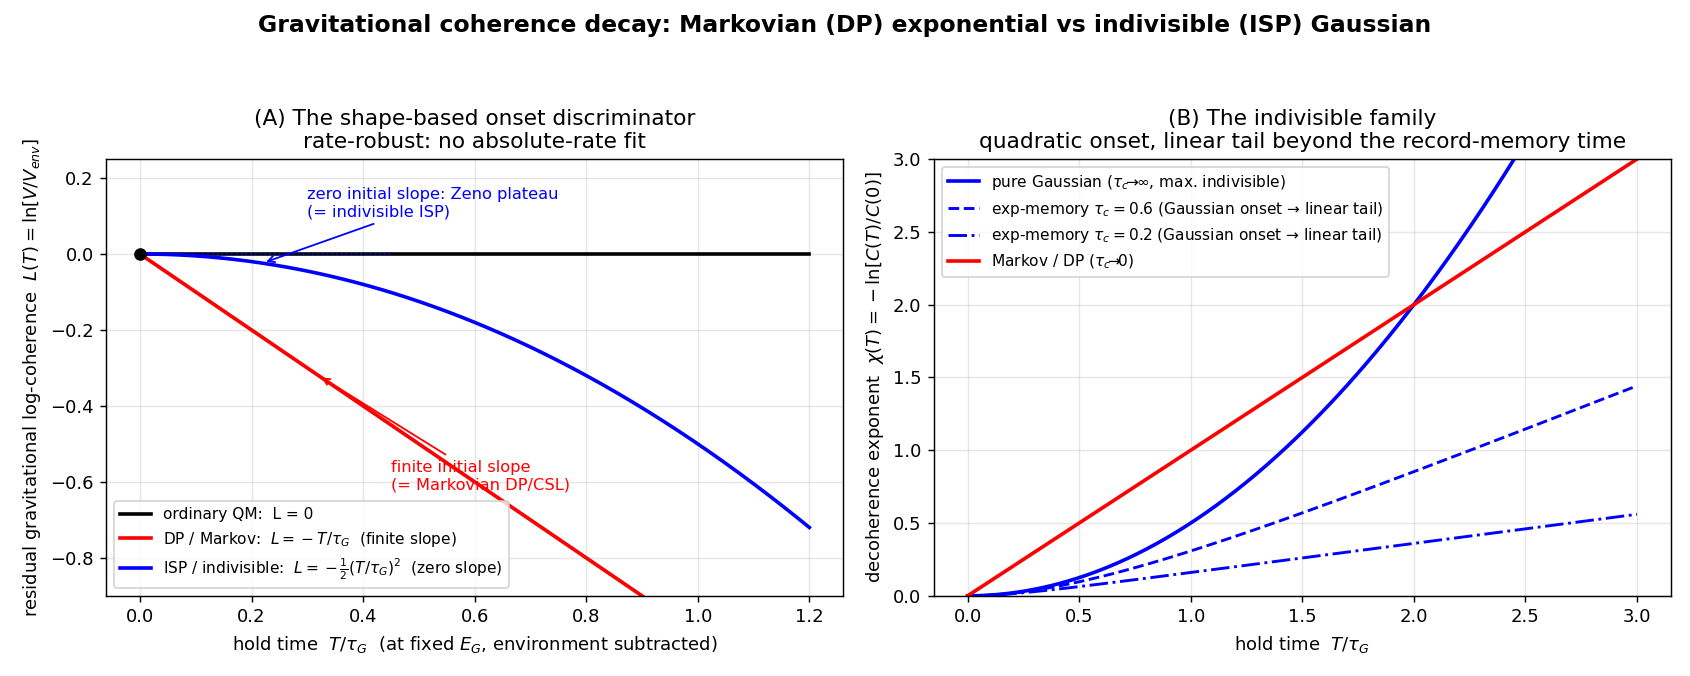
\includegraphics[width=0.98\linewidth]{fig1_onset.png}
\caption{The shape-based discriminator. \textbf{(A)}~Residual gravitational log-coherence
$L(T)=\ln[V/V_{\rm env}]$ at fixed $E_G$: ordinary quantum mechanics gives $L=0$; Markovian DP/CSL a
straight line through the origin (finite initial slope); the indivisible finite-memory channel a
parabola tangent to the axis (zero initial slope, a Zeno-like plateau). The discriminating feature is
the leading power of $T$, which needs no absolute-rate calibration. \textbf{(B)}~The decoherence
exponent $\chi(T)=-\ln[C(T)/C(0)]$ for the finite-memory family: a pure Gaussian
($\tau_c\!\to\!\infty$), exponential-memory kernels with finite $\tau_c$ (Gaussian onset crossing to
a linear, DP-slope tail beyond the record-memory time $\tau_c$), and the Markovian DP limit
($\tau_c\!\to\!0$). The benchmark closure sits at $\tau_c\sim\tau_G$.}
\label{fig:onset}
\end{figure}

\paragraph{How large is the effect, and what precision does it need?} At fixed $E_G$ the two
candidate visibility curves are $V_{\rm exp}=e^{-x}$ (Markovian DP) and $V_{\rm Gauss}=e^{-x^2/2}$
(benchmark ISP), with $x=T/\tau_G$ (Table~\ref{tab:visibility}). The curves separate most near
$T\approx0.65\,\tau_G$, where they differ by $\Delta V\approx0.29$---about 30\% of the initial
visibility. Discriminating the two shapes at the few-$\sigma$ level therefore calls for a visibility
resolution of a few percent across the window $T\in[0.3,1.5]\,\tau_G$ (with $\tau_G$ of order seconds
to hours for the masses of Sec.~\ref{sec:thresholds})---demanding, but on the trajectory of current
mesoscopic-superposition programmes. In the \emph{defined} observable $L=\ln(V/V_{\rm env})$ the
separation is exactly $\Delta L=x-x^2/2$, which peaks at $x=1$ (i.e.\ $T=\tau_G$, $\Delta L=0.5$);
since interferometric data are usually analysed in log-visibility, $T\approx\tau_G$ is the natural
probe time.

\begin{table}[h]
\centering
\caption{Candidate visibility curves and their separation, $x=T/\tau_G$.}\label{tab:visibility}
\begin{tabular}{cccc}
\hline\hline
$x=T/\tau_G$ & $V_{\rm exp}$ & $V_{\rm Gauss}$ & $\Delta V$ \\
\hline
0.3 & 0.74 & 0.96 & 0.21 \\
0.5 & 0.61 & 0.88 & 0.28 \\
0.65 & 0.52 & 0.81 & 0.29 \\
1.0 & 0.37 & 0.61 & 0.24 \\
1.5 & 0.22 & 0.32 & 0.10 \\
\hline\hline
\end{tabular}
\end{table}

A non-Markovian \emph{environment} produces the same quadratic onset~\cite{R21,R22}, so curvature alone
does not establish a gravitational origin---only the \emph{scaling} with $E_G$ does, and the
discriminating power lies in knobs that move $E_G$ while leaving the environment fixed:
\begin{itemize}
\item \textbf{Density.} Gravitational decoherence scales as $E_G\propto\rho^2$ (harmonic
$\propto\rho^2 R^3 d^2$, saturated $\propto\rho^2 R^5$), whereas gas-collision and blackbody
decoherence depend on external geometry, surface, polarizability, pressure and temperature but are
essentially \emph{blind to bulk mass density} at fixed external size~\cite{R16} (with one honest
caveat: dielectric response correlates with density across real materials via Clausius--Mossotti, so
the blackbody channel's $\rho$-blindness is approximate, and its discrimination leans on the
internal-temperature knob below). Comparing same-size,
same-shape particles of very different density isolates gravity by a $\rho^2$ law no environmental
channel mimics.
\item \textbf{Common-mode subtraction.} Run a high-$E_G$ and a low-$E_G$ configuration in the
\emph{same} chamber, vacuum and thermal/seismic environment and subtract: vibration, gas and blackbody
backgrounds are largely common-mode and cancel, leaving the gravitational differential---the standard
precision-measurement strategy.
\item \textbf{Calibrate by knob.} Gas decoherence scales with pressure and blackbody with internal
temperature, while gravity is pressure- and temperature-independent; mapping the onset curvature
versus $P$ and $T$ and extrapolating $P\to0$, $T\to0$ removes those channels.
\end{itemize}
Two further fingerprints sharpen this. (a)~Gravitational $E_G(d)$ saturates at the \emph{object size}
$d\sim R$, whereas environmental channels saturate at thermal or scattering wavelengths.
(b)~\textbf{Plateau duration.} The quadratic (Zeno) plateau of \emph{any} finite-memory channel lasts
only until its correlation time; the gravitational plateau persists to $\tau_c\sim\tau_G$
(seconds--hours), whereas gas- and blackbody-bath correlation times are microseconds or shorter---so a
quadratic onset \emph{surviving to macroscopic hold times} cannot be a fast environmental bath, which
would already have crossed over to its linear tail. This cleanly excludes the \emph{fast} baths; it
does \textbf{not} by itself exclude slow, low-frequency backgrounds (structural $1/f$ noise, drift),
which can sustain a long plateau of their own---those are removed not by plateau duration but by the
$E_G$-scaling (density) lever above, which no environmental channel reproduces. None of this is easy---it is a long-term programme, not a near-term
measurement---but the gravitational channel is identified by a \emph{joint} scaling (with $\rho$, $d$,
$P$, $T$) that no single environmental source reproduces.

\paragraph{A second axis: distinguishing ISP from the whole collapse-model family.} The onset shape
separates ISP from any \emph{Markovian} collapse model, but several related theories must be told
apart at once, and they are distinguished by \emph{two} axes---the onset shape and the scaling of the
rate. (Both axes are plain, non-relativistic physics: indivisibility supplies the onset, and the
\emph{inherited} DP scale --- ansatz (M2), not an ISP derivation --- supplies the $E_G$ scaling;
the relativistic extension adds nothing here.)
This cell---finite-memory gravitational decoherence---is reached by no Markovian or non-gravitational
model (Table~\ref{tab:twoaxis}).

\begin{table}[h]
\centering
\caption{The two-axis classification: onset shape $\times$ rate scaling.}\label{tab:twoaxis}
\begin{tabular}{lccc}
\hline\hline
Theory & Fundamental decay? & Onset shape & Rate scaling \\
\hline
Unitary QM / QFT & no & --- (only $\Gamma_{\rm env}$) & --- \\
Schr\"odinger--Newton (mean-field)~\cite{R24} & no---a phase/freq.\ \emph{shift} & --- & grav., but a shift \\
CSL / GRW (Markovian, non-grav.)~\cite{R4,R5} & yes & exponential & params $(\lambda,r_C)$, not $E_G$ \\
Di\'osi--Penrose (Markovian, grav.)~\cite{R1,R2} & yes & exponential & gravitational $E_G$ \\
\textbf{ISP finite-memory (this work)} & \textbf{yes} & \textbf{Gaussian} & \textbf{gravitational $E_G$} \\
\hline\hline
\end{tabular}
\end{table}

A two-axis measurement settles it. \textbf{Axis 1 (onset shape)}, above, separates ISP from the
Markovian models (exponential vs Gaussian). \textbf{Axis 2 (rate scaling):} vary the mass $M$,
separation $d$, and geometry, and test whether the rate tracks the gravitational self-energy $E_G$
(the Di\'osi--Penrose form, $\propto G$) or the CSL parameters ($\lambda,r_C$, with a fixed
$\sim10^{-7}\,$m length scale and a different geometry dependence); the Schr\"odinger--Newton
alternative appears instead as a deterministic frequency \emph{shift} with no decay, testable by
the proposed optomechanical experiments~\cite{R24}. A result in the (Gaussian onset) $\times$ (gravitational
$E_G$-scaling) cell supports the ISP-motivated non-Markovian gravitational hypothesis---without
uniquely establishing ISP (see the limits below)---and simultaneously excludes Markovian DP
(exponential), CSL/GRW (wrong scaling), Schr\"odinger--Newton (shift, not decay), and unitary QM (no
decay).

\paragraph{A third axis: the non-Gaussian fingerprint of discrete records.} A \emph{coloured}
(non-Markovian) \emph{gravitational} collapse---Gaussian noise with the same $E_G$-scaling---would
share both cells above. A third axis separates it, and it too lives in the visibility curve. Generic
coloured noise is Gaussian by construction, so its coherence is exactly the second-cumulant result
$C(T)=e^{-\chi(T)}$ (monotone, log-convex); the division-event process of Sec.~\ref{subsec:micro} is a
\emph{jump} process and is non-Gaussian,
\begin{equation}
\ln|C(T)|=-\chi(T)+\frac{\kappa_4(T)}{24}-\cdots,
\end{equation}
where the Gaussian alternative has all cumulants $\kappa_n=0$ for $n\ge3$. In the long-memory regime
$T\lesssim\tau_c$ the coherence is the \emph{characteristic function} of the per-division
mismatch-energy distribution, $C(T)=\langle e^{i\delta E\,T/\hbar}\rangle$: a Gaussian $p(\delta E)$
reproduces the Gaussian onset, while a discrete, branch-selecting $\delta E$ produces non-Gaussian
structure---up to coherence \emph{revivals} ($C(T)=\cos(\sigma_E T/\hbar)$ for $\delta E=\pm\sigma_E$),
which no monotone $e^{-\chi}$ can produce. The effect is not parametrically small: at $T\sim\tau_G$ the
leading correction is set by the excess kurtosis of $p(\delta E)$ (for bimodal $\delta E=\pm\sigma_E$
the quartic term is $x^4/12$ against the quadratic $x^2/2$: $17\%$ of the onset exponent at
$x = \sigma_E T/\hbar = 1$, equivalently $\approx8\%$ of $\chi\approx1$ at the closure point ---
both conventions stated since an earlier draft quoted only the second), and it occupies the \emph{same}
observable window as the onset, washing out only in the white-noise limit. Since the discreteness of
records is precisely the ISP content a continuum (Gaussian) theory lacks, a measured departure of
$C(T)$ from the pure form $e^{-\chi(T)}$---a $T^4$ term, or non-monotonicity---is a \emph{positive}
signature of discrete record formation. The three axes nest: (1)~onset shape (linear vs quadratic)
falsifies strict Markovian DP/CSL; (2)~rate scaling ($E_G$ vs $\lambda,r_C$) separates gravitational
from non-gravitational; (3)~non-Gaussianity (a $T^4$ term, up to revivals) separates discrete-record
from Gaussian coloured gravitational collapse. Axis~3 rides on $p(\delta E)$ being non-Gaussian---
unpredicted from first principles (a limitation, below)---and narrows the field to
\emph{discrete-record} models rather than singling out ISP uniquely.

\paragraph{Honest limits of the test.} (i)~A non-Markovian \emph{gravitational} collapse
model could share the first two cells; axis~3 separates the Gaussian (coloured-noise) version by its
absent non-Gaussian fingerprint, narrowing the degeneracy to \emph{discrete-record} gravitational
models, which are distinguished from ISP only at the level of motivation and ontology. (A \emph{coloured}
(non-Markovian) CSL~\cite{R10} can mimic the Gaussian onset but not the gravitational $E_G$-scaling,
so the second axis still separates that case.) (ii)~Axis~2 is a \emph{campaign}: the $E_G$-scaling
must be mapped across a range of $M,d$, geometry, not read from one curve. (iii)~The test
presupposes the fundamental channel exists at all---if nature is exactly unitary, every row collapses
to ``no decay'' and ISP is empirically QM. (iv)~The regime is at the frontier of
mesoscopic-superposition sensitivity, not yet in hand. Within these limits the test upgrades
the discriminator from ``ISP vs.\ standard quantum mechanics'' to ``ISP vs.\ the entire
collapse/decoherence family.''

\section{Numerical thresholds and experimental platforms}\label{sec:thresholds}

We quote thresholds for a rigid homogeneous sphere of mass $M$, radius $R$, density $\rho$,
coherently separated by $d$. For $d\ll R$ the mismatch energy is harmonic,
\begin{equation}
E_G\simeq\tfrac12 M\omega_G^2 d^2,\qquad \omega_G^2=\frac{4\pi G\rho}{3},
\end{equation}
while for object-scale separations it saturates at the self-energy scale
\begin{equation}
E_G^{\rm sat}\simeq\frac{6}{5}\frac{GM^2}{R}.
\end{equation}
Using $\rho=2000\,\mathrm{kg\,m^{-3}}$, the saturated threshold mass that decoheres in time $T$
(i.e.\ $\tau_G=T$) is
\begin{equation}
M_{\rm thr}^{\rm sat}(T)=\left[\frac{\hbar}{\tfrac65 G\,(4\pi\rho/3)^{1/3}\,T}\right]^{3/5}.
\end{equation}
Representative values are given in Table~\ref{tab:thresholds} (saturated regime, $d\gtrsim R$;
order-of-magnitude DP-energy thresholds at $\tau_G=T$, not feasibility estimates). For an actual
experiment the self-energy must be evaluated numerically from the measured density profile and branch
geometry; the harmonic and saturated formulas above are limiting estimates used only to locate the
relevant mass--time scale. These mass and separation windows coincide with the targets of current and
proposed mesoscopic-superposition experiments~\cite{R16,R17,R19,R23,R26,R27,R28}. Three platform
classes are natural hosts for the onset-shape test:
\begin{itemize}
\item \textbf{Levitated nanosphere interferometry.} Neutral dielectric nanospheres in ultra-high
vacuum, prepared in spatial superposition and recombined; ground-state cooling and control of such
particles is now routine~\cite{R27,R28}.
\item \textbf{Mesoscopic matter-wave interferometry.} Large-molecule and cluster interferometers,
where macroscopicity has been advanced systematically, now beyond 25~kDa~\cite{R16,R23,R26}.
\item \textbf{Mechanical cat states / optomechanics.} Superpositions of a massive mechanical
element~\cite{R19}, including the gravity-mediated-entanglement geometries~\cite{R17,R18} in which
$E_G$ can be tuned by separation.
\end{itemize}
In every case the experimental strategy for the discriminator is identical: hold the object,
temperature, vacuum, and pulse sequence fixed, vary $E_G$ (e.g.\ through the separation $d$), and
examine whether the gravitational contribution to $\ln V$ enters linearly or quadratically in the
hold time.

\begin{table}[h]
\centering
\caption{Saturated threshold mass and radius decohering in time $T$ ($\rho=2000\,\mathrm{kg\,m^{-3}}$).}
\label{tab:thresholds}
\begin{tabular}{cccc}
\hline\hline
$T$ & $M_{\rm thr}$ (kg) & $M_{\rm thr}$ (amu) & $R_{\rm thr}$ \\
\hline
$1\,\mu$s & $3.1\times10^{-12}$ & $1.9\times10^{15}$ & $7.2\,\mu$m \\
$1\,$ms & $4.9\times10^{-14}$ & $2.9\times10^{13}$ & $1.8\,\mu$m \\
$1\,$s & $7.7\times10^{-16}$ & $4.6\times10^{11}$ & $452\,$nm \\
$100\,$s & $4.9\times10^{-17}$ & $2.9\times10^{10}$ & $180\,$nm \\
$1\,$h & $5.7\times10^{-18}$ & $3.4\times10^{9}$ & $88\,$nm \\
\hline\hline
\end{tabular}
\end{table}

\section{The record-memory time}\label{sec:tauc}

The new scale $\tau_c$ is the autocorrelation time of the gravitational mismatch---in the ISP
language, the mean spacing between division events of the gravitational record channel.
Section~\ref{subsec:micro} fixed it for the \emph{channel-intrinsic} case---where the division event
\emph{is} the record stabilization---at $\tau_c\approx1.65\,\tau_G$ via the record-stabilization fixed
point $\chi(\tau_c)\approx1$, so that the memory time and the stabilization time coincide up to an
$O(1)$ factor,
\begin{equation}
\tau_c\sim\tau_G=\hbar/E_G.
\end{equation}
That value is not unique, however: it presumes the channel is governed by its own stabilization time,
whereas other physical scales are conceivable. The candidate scales and their consequences are
given in Table~\ref{tab:tauc}.

Two considerations show the channel does not generically slide to the Markovian floor, and that
$\tau_c\gtrsim\tau_G$ is \emph{strongly motivated} rather than freely chosen (not forced: the
information-gating premise below --- that record formation requires order-unity distinguishability ---
is itself a hypothesis). First, \textbf{records are information-gated}:
a division event is the gravitational field committing to a which-branch record, and no record can form
before the branches are distinguishable---at the light-crossing time the accumulated distinguishability
is $\chi(R/c)\sim(R/c\,\tau_G)^2\sim10^{-30}$, so there is nothing to record, and the record time is
bounded below by the time to reach order-unity distinguishability, $\tau_c\gtrsim\tau_G$. Second,
\textbf{a fast clock does not recover DP} at the physical fluctuation amplitude $\sigma_E\sim E_G$: the
decoherence slope $\sigma_E^2\tau_c/\hbar^2$ is then smaller than the DP slope $1/\tau_G$ by
$\tau_c/\tau_G\sim10^{-15}$, a quantum-Zeno freeze, not the DP exponential. (Recovering DP as
$\tau_c\to0$ requires holding the noise \emph{power} $\sigma_E^2\tau_c$ fixed, hence
$\sigma_E\to\infty$; see Sec.~\ref{sec:limits}.) Equivalently, requiring the decoherence to be
DP-\emph{sized} at $\sigma_E\sim E_G$ forces $\tau_c\gtrsim\tau_G$: the onset curvature reaches order
unity at $T\sim\tau_G$ only if the crossover has not already turned the decay into its slow linear tail.

The honest verdict is that \emph{finite memory} forces the decay away from a strict exponential---and
indivisibility motivates the finite memory---with $\tau_c$ tied to the gravitational scale two
ways: by the Sec.~\ref{subsec:micro} fixed point and by information-gating.  (A third consideration
sometimes invoked---that an \emph{observable} DP-scale effect requires $\tau_c$ in the measurement
window---is experimental-design reasoning, not physics: nature is not obliged to put $\tau_c$ in the
observable window, and we do not count it as a pinning.) The DP-Markovian limit is the unphysical $\sigma_E\to\infty$ corner. The
channel-intrinsic and gravitational-dynamical candidates both place the crossover within the observable
window ($\tau_c$ of order seconds to hours for the masses in Sec.~\ref{sec:thresholds}), so the
Gaussian onset is accessible.

\begin{table}[h]
\centering
\caption{Candidate record-memory times and their observational consequence.}\label{tab:tauc}
\begin{tabular}{lll}
\hline\hline
candidate $\tau_c$ & origin & consequence \\
\hline
$\hbar/E_G=\tau_G$ & channel-intrinsic (division $=$ stabilization) & Gaussian onset near $T\sim\tau_G$ \\
$\sqrt{3/4\pi G\rho}=1/\omega_G$ & gravitational dynamical time (density only) & $\sim10^3\,$s for rock: observable \\
$R/c$ & light-crossing (microphysical floor) & $\sim10^{-15}\,$s: Zeno-suppressed at fixed $\sigma_E$ ($\sigma_E\!\to\!\infty$ for DP) \\
\hline\hline
\end{tabular}
\end{table}

\section{Spontaneous radiation and existing bounds}\label{sec:radiation}

The parameter-free DP model is experimentally excluded. Donadi et al.~\cite{R8} searched underground
at the Gran Sasso laboratory for the spontaneous electromagnetic radiation that collapse-driven
charge diffusion would produce, found no excess, and tightened the bound on the effective nuclear
mass-density size by about three orders of magnitude, ruling out the simplest DP model; current
bounds on the wider collapse-model family are reviewed in~\cite{R25}.

The radiation bound constrains the model's regularization, not its prediction. The DP noise carries a
short-distance regularization length $R_0$, and two effects are set by \emph{different} scales:
\begin{itemize}
\item the \textbf{decoherence} of the superposition is collective---the gravitational self-energy of
the displaced mass distribution, $E_G\approx(6/5)GM^2/R$, set by the \emph{object size} $R$ and
\textbf{independent of $R_0$} (every nucleon separation exceeds $R_0$);
\item the \textbf{spontaneous emission and heating} of bulk matter are a per-nucleon momentum
diffusion, $\propto 1/R_0^3$, set by the regularization $R_0$.
\end{itemize}
These decouple: for any nanoscale object the structural (decoherence) term exceeds the per-nucleon term
by many orders, so matching the decoherence does \emph{not} fix the emission. The Gran Sasso X-ray
search therefore bounds $R_0$---giving $R_0\gtrsim0.5$~\AA{} for white DP~\cite{R8}, with
spontaneous-heating and mechanical bounds two orders weaker ($R_0\gtrsim5\times10^{-13}$~m) but robust
to non-Markovian generalizations~\cite{R25}---and none of these touch the ($R_0$-independent)
decoherence the interferometer measures.

The finite-memory modification only \emph{helps} on the emission side. Emission at the photon frequency
is governed by the noise spectral density there---a noise band-limited to $1/\tau_c$ is adiabatic on the
keV photon timescale and carries no keV quanta to deposit---so with $S(\omega)=S(0)/[1+(\omega\tau_c)^2]$
the temporal cutoff suppresses keV emission by $(E_G/\hbar\omega_{\rm keV})^2\sim10^{-36}$ relative to
white DP, the gravitational mismatch energy being the natural emission cutoff. This Lorentzian (rather
than exponential) tail is the \emph{least}-suppressed case, forced by the cusp the discrete division
events put in the kernel at the origin ($K'(0^+)=-\sigma_E^2/\tau_c$, for any waiting-time law); even
this worst case is suppressed by $10^{-36}$; with sharp lab-time resets the emission margin would
read out the division microstructure of Sec.~\ref{subsec:micro}, though a covariant completion
smooths the kernel's cusp on timescales $\lesssim R/c$ and weakens that readout while strengthening
the suppression (see the Note added). In this sense the finite memory acts as a \emph{temporal}
ultraviolet regulator: the band-limit $1/\tau_c$ curtails the high-frequency radiation that the flat
white-noise spectrum would make divergent---the role the \emph{spatial} smearing $R_0$ plays for the
static self-energy. The two regulators act on \emph{different} sectors and do not substitute for one
another: $\tau_c$ does not soften the ($R_0$-set) spatial self-energy, nor the (zero-frequency,
$S(0)$-set) heating, which is precisely why the heating bound remains the robust one above. (The
zero-frequency emission term
sometimes invoked for collapse models was shown to be a non-normalizable-state artifact that vanishes
for wave packets~\cite{R9,R10}.) The finite-memory channel thus inherits standard DP's consistency with
the radiation and heating bounds---at worst identically, and at the keV frequencies actually searched,
more comfortably---while changing only the \emph{onset shape} of the decoherence, not its magnitude or
radiation phenomenology.  (One extrapolation is used here and flagged: the bulk-matter emitters of the
radiation searches carry no prepared superposition, while $\tau_c$ in this model is tied to the
two-branch configuration of an interferometer --- the effective-description caveat of
Sec.~\ref{subsec:micro}.  The conclusion is insensitive to this: \emph{any} $\tau_c$ far above
attoseconds kills keV emission, and the zero-frequency heating bound is inherited at worst
identically.)

\section{Discussion: scope and limitations}\label{sec:limits}

We state the boundaries of the result plainly.
\begin{itemize}
\item \textbf{The energy scale is DP's, not new.} The contribution is the non-exponential
\emph{shape} and its falsifiable onset, not the magnitude $\tau_G=\hbar/E_G$, which is taken over
from~\cite{R1,R2,R3}.
\item \textbf{The coefficient inherits DP's ansatz dependence.} Whether the Gaussian onset time
equals $\hbar/E_G$ exactly depends on $\tau_c$ and $\sigma_E$ (generally $\tau_{\rm
Gauss}=\sqrt{\tau_c\,\tau_G}$); only the quadratic \emph{shape} is assumption-light.
\item \textbf{The quadratic onset is generic to non-Markovianity.} It is shared by coloured-noise CSL
and by non-Markovian environmental decoherence~\cite{R10,R21,R22}. Observing it would falsify
\emph{strict} Markovian DP/CSL and be evidence for a non-Markovian fundamental channel consistent
with ISP, but would not by itself single out ISP among non-Markovian models.
\item \textbf{$\tau_c$ is a genuinely new parameter.} The division-event model
(Sec.~\ref{subsec:micro}) pins it to $\approx1.65\,\tau_G$ via the record-stabilization fixed point, but
this rests on the renewal-reset ansatz, and Sec.~\ref{sec:tauc} lists other candidate scales that
interpolate toward the Markovian limit.
\item \textbf{The analysis is non-relativistic throughout.}  Kernels are correlated in laboratory
time, energies are Newtonian, and the platforms are slow: nothing here claims Lorentz covariance,
and the covariant completion of a finite-memory kernel is a separate problem (see the Note added).
\item \textbf{The DP limit is the white-noise limit, not $\tau_c\to0$ at fixed amplitude.} At fixed
$\sigma_E$ the $\tau_c\to0$ limit gives vanishing decoherence, not DP; the strict DP law requires
holding the noise power $\sigma_E^2\,\tau_c$ fixed. The clean ``Gaussian onset at $\tau_G$ with a
DP-slope tail'' picture holds at the self-consistent point $\tau_c\sim\tau_G$, $\sigma_E\sim E_G$
(Secs.~\ref{subsec:hierarchy}, \ref{subsec:micro} and~\ref{sec:tauc}), which is an ansatz, not a theorem.
\item \textbf{Environmental non-Markovianity must be controlled.} Because a non-Markovian
\emph{environment} can also produce a quadratic onset, the test requires that the residual after
environmental subtraction be attributable to the gravitational channel---most cleanly demonstrated by
its scaling with $E_G$ at fixed environment.
\end{itemize}
Within these bounds, the result is a concrete, falsifiable alternative to the Markovian DP law,
motivated by a specific and independently-motivated stochastic ontology~\cite{R11,R12}, and testable
with the same platforms already pursuing DP~\cite{R16,R17,R19,R23}.

\section{Conclusion}\label{sec:conclusion}

Treating gravitational decoherence as a process in an indivisible (non-Markovian) stochastic dynamics
replaces the Di\'osi--Penrose exponential with a non-exponential, Gaussian-onset coherence
decay---at the self-consistent point $\tau_c\sim\tau_G$, $\sigma_E\sim E_G$, at the same gravitational
energy scale---with the strict DP exponential recovered in the white-noise limit. The distinction is
experimentally sharp and rate-robust: the discriminator is the leading power of $T$ in the residual
gravitational log-coherence---linear for Markovian collapse, quadratic for the indivisible
channel---not an absolute rate. The benchmark model identifies the crossover scale $\tau_c$ with the
DP time $\tau_G$---other choices interpolate between a visibly non-Markovian onset and the Markovian
DP limit---and with $\tau_c\sim\tau_G$ the effect lies within reach of mesoscopic-superposition
experiments. The robust content is conceptual and methodological---that the DP exponential is a
Markovian idealization, and that the onset \emph{shape} together with its $E_G$-scaling is a
falsifiable discriminator for \emph{any} finite-memory gravitational decoherence, separable by a
density lever and common-mode subtraction from environmental backgrounds. The radiation and heating
bounds constrain only the model's regularization length and decouple from the ($R_0$-independent)
decoherence, so the finite-memory channel inherits standard DP's consistency with them; what it adds to
standard DP is the onset \emph{shape} alone---now grounded (Sec.~\ref{subsec:micro}) in the
division-event structure of the indivisible process.


\section*{Note added (11 June 2026)}

After this paper was completed, companion work within the same
program (manuscript in preparation: \emph{Interacting
Tomonaga--Schwinger integrability of indivisible division-event
dynamics}; archived with the program repository accompanying this
deposit) examined the \emph{relativistic} completion of
finite-memory collapse noise and reached two results that bear on,
without modifying, the present analysis.  (i) A frame-fixed
correlation time --- the form used here, $K(s)\propto e^{-|s|/\tau_c}$
in laboratory time --- is not Lorentz-covariant; a covariant memory
must correlate in the invariant interval, $K = f\bigl((x-y)^2\bigr)$,
and finiteness of the induced energy production requires its
spectrum to decay faster than any power (a quartic-exponential
class $\hat f(q)\propto e^{-q^4/\beta^4}$ suffices), while
Lorentzian/Ornstein--Uhlenbeck spectra remain ultraviolet-divergent
relativistically.  (ii) This does not alter the present paper's results,
whose scope is explicitly non-relativistic
(Sec.~\ref{sec:limits}), with one qualification: a covariant
$f\bigl((x-y)^2\bigr)$ restricted to a laboratory worldline is a
smooth even function of the time lag, so it reproduces the
exponential kernel used here only up to a covariant smoothing of
the kernel's cusp at the origin on timescales $\lesssim R/c$ ---
which leaves the onset-shape discriminator untouched (it is a
property of the finite-memory \emph{class}, not of the kernel's
detailed shape) and only \emph{strengthens} the high-frequency
emission suppression of Sec.~\ref{sec:radiation}, while weakening
that section's microstructure-readout remark, which we have
qualified accordingly.  What the
companion result adds is a sharpening at the program level: if the
quadratic onset is observed, the covariant completion of the
inferred memory is constrained to the smooth (faster-than-power-law)
spectral class, not merely to ``coloured noise.''

\begin{thebibliography}{99}

\bibitem{R1} R. Penrose, \emph{On gravity's role in quantum state reduction}, Gen. Relativ. Gravit. \textbf{28}, 581 (1996).
\bibitem{R2} L. Di\'osi, \emph{Models for universal reduction of macroscopic quantum fluctuations}, Phys. Rev. A \textbf{40}, 1165 (1989).
\bibitem{R3} L. Di\'osi, \emph{A universal master equation for the gravitational violation of quantum mechanics}, Phys. Lett. A \textbf{120}, 377 (1987).
\bibitem{R4} G. C. Ghirardi, A. Rimini, T. Weber, \emph{Unified dynamics for microscopic and macroscopic systems}, Phys. Rev. D \textbf{34}, 470 (1986).
\bibitem{R5} G. C. Ghirardi, P. Pearle, A. Rimini, \emph{Markov processes in Hilbert space and continuous spontaneous localization of systems of identical particles}, Phys. Rev. A \textbf{42}, 78 (1990).
\bibitem{R6} A. Bassi, G. C. Ghirardi, \emph{Dynamical reduction models}, Phys. Rep. \textbf{379}, 257 (2003).
\bibitem{R7} A. Bassi, K. Lochan, S. Satin, T. P. Singh, H. Ulbricht, \emph{Models of wave-function collapse, underlying theories, and experimental tests}, Rev. Mod. Phys. \textbf{85}, 471 (2013).
\bibitem{R8} S. Donadi, K. Piscicchia, C. Curceanu, L. Di\'osi, M. Laubenstein, A. Bassi, \emph{Underground test of gravity-related wave function collapse}, Nat. Phys. \textbf{17}, 74 (2021).
\bibitem{R9} S. L. Adler, A. Bassi, S. Donadi, \emph{On spontaneous photon emission in collapse models}, J. Phys. A: Math. Theor. \textbf{46}, 245304 (2013).
\bibitem{R10} M. Carlesso, L. Ferialdi, A. Bassi, \emph{Colored collapse models from the non-interferometric perspective}, Eur. Phys. J. D \textbf{72}, 159 (2018).
\bibitem{R11} J. A. Barandes, \emph{The stochastic-quantum correspondence}, arXiv:2302.10778 (2023).
\bibitem{R12} J. A. Barandes, \emph{The stochastic-quantum theorem}, arXiv:2309.03085 (2023).
\bibitem{R14} W. H. Zurek, \emph{Decoherence, einselection, and the quantum origins of the classical}, Rev. Mod. Phys. \textbf{75}, 715 (2003).
\bibitem{R15} H.-P. Breuer, F. Petruccione, \emph{The Theory of Open Quantum Systems} (Oxford University Press, 2002).
\bibitem{R16} M. Arndt, K. Hornberger, \emph{Testing the limits of quantum mechanical superpositions}, Nat. Phys. \textbf{10}, 271 (2014).
\bibitem{R17} S. Bose et al., \emph{Spin entanglement witness for quantum gravity}, Phys. Rev. Lett. \textbf{119}, 240401 (2017).
\bibitem{R18} C. Marletto, V. Vedral, \emph{Gravitationally induced entanglement between two massive particles is sufficient evidence of quantum effects in gravity}, Phys. Rev. Lett. \textbf{119}, 240402 (2017).
\bibitem{R19} W. Marshall, C. Simon, R. Penrose, D. Bouwmeester, \emph{Towards quantum superpositions of a mirror}, Phys. Rev. Lett. \textbf{91}, 130401 (2003).
\bibitem{R20} A. Bassi, A. Gro\ss ardt, H. Ulbricht, \emph{Gravitational decoherence}, Class. Quantum Grav. \textbf{34}, 193002 (2017).
\bibitem{R21} H.-P. Breuer, E.-M. Laine, J. Piilo, B. Vacchini, \emph{Colloquium: Non-Markovian dynamics in open quantum systems}, Rev. Mod. Phys. \textbf{88}, 021002 (2016).
\bibitem{R22} B. Misra, E. C. G. Sudarshan, \emph{The Zeno's paradox in quantum theory}, J. Math. Phys. \textbf{18}, 756 (1977).
\bibitem{R23} S. Nimmrichter, K. Hornberger, \emph{Macroscopicity of mechanical quantum superposition states}, Phys. Rev. Lett. \textbf{110}, 160403 (2013).
\bibitem{R24} A. Gro\ss ardt, J. Bateman, H. Ulbricht, A. Bassi, \emph{Optomechanical test of the Schr\"odinger-Newton equation}, Phys. Rev. D \textbf{93}, 096003 (2016); arXiv:1510.01696.
\bibitem{R25} M. Carlesso, S. Donadi, L. Ferialdi, M. Paternostro, H. Ulbricht, A. Bassi, \emph{Present status and future challenges of non-interferometric tests of collapse models}, Nat. Phys. \textbf{18}, 243 (2022); arXiv:2203.04231.
\bibitem{R26} Y. Y. Fein, P. Geyer, P. Zwick, F. Kia{\l}ka, S. Pedalino, M. Mayor, S. Gerlich, M. Arndt, \emph{Quantum superposition of molecules beyond 25 kDa}, Nat. Phys. \textbf{15}, 1242 (2019).
\bibitem{R27} U. Deli\'c, M. Reisenbauer, K. Dare, D. Grass, V. Vuleti\'c, N. Kiesel, M. Aspelmeyer, \emph{Cooling of a levitated nanoparticle to the motional quantum ground state}, Science \textbf{367}, 892 (2020).
\bibitem{R28} C. Gonz\'alez-Ballestero, M. Aspelmeyer, L. Novotny, R. Quidant, O. Romero-Isart, \emph{Levitodynamics: Levitation and control of microscopic objects in vacuum}, Science \textbf{374}, eabg3027 (2021); arXiv:2111.05215.

\end{thebibliography}

\end{document}
